\documentclass[10pt,a4paper]{article}
\usepackage[utf8]{inputenc}
\usepackage{amsmath}
\usepackage{amsfonts}
\usepackage{amssymb}
\usepackage{natbib}
\usepackage{url}
\usepackage{pgf}
\usepackage{tikz}
\usepackage{listings}

\usetikzlibrary{fit}
\usetikzlibrary{positioning}
\usetikzlibrary{arrows,automata}

\tikzstyle{state} = [draw, fill=blue!20, text width=5cm,
text centered, minimum height=2.5em, fill=white!20]
\tikzstyle{subject} = [state, fill=blue!20]

\author{Tobias Arrskog}
\title{Heimdall}

\bibliographystyle{plain}

\begin{document}

\section{Introduction}
Heimdall began its existence as a Google Summer of Code project in 2012 for xbmc media center. The goal of the project was to research the possibility to create a new engine which would handle the information extraction more generically (in terms of media content) and more efficiently. Another goal was to create something which was not bound to xbmc, so it could be used by the entire ecosystem.

\section{Goal}

\begin{description}
	\item[Generalized] adding a new media type should be trivial, no part of the core should be bound by media types.
	\item[Dynamic fields] what fields is of interest is not tied to the engine, any scraper may add metadata as it sees fit. The user of the engine (xbmc, skinners etc) may choose what data it understands but scrapers can emit all type of data it wants.
	\item[Parallelism] as much as possible needs to be parallelism friendly, ideally not only between files but all parts of scraping of a file too.
\end{description}

\section{Nomenclature}

\begin{description}
	\item[Subject] The entity targeted to find more information about.
	\item[Object] Can be either a literal or a url locating a subject. So it can be loosely linked data only associated with one subject or it can be another subject.
	\item[Predicate] A link/edge between a subject and object
\end{description}

Subject, predicate and object are the same as those of the W3C rdf \cite{w3c-rdf} and semantic web \cite{wiki-semantic-web} \cite{w3c-semantic-web}.

\begin{description}
	\item[Metadata] The term is in short the same as subject, predicate and object. Usually when using the term metadata however its only speaking of a single subject and all of its predicate and objects, or a single subject with a single predicate, object.
	\item[Resource] Anything holding data, which could be used to extract metadata from. A resource must be identified via URL and is a resource in the same definitions as that of the W3C standard in regards to URI and URL \cite{w3c-url} \cite{w3c-uri}.
\end{description}

\section{Design}
Heimdall uses constraints, both soft and hard, to create a pipeline for a given subject. The subject given to Heimdall may expose differing properties and the engine will create a suitable pipeline during the extraction process. To find the constraints Heimdall will use the subjects predicate and objects along with what tasks supplies and demands.

As an example a task might have a \emph{demand} on \emph{title} of a subject, without this title the task cannot run, thus creating a hard \emph{constraint} between this subject task and the subject. If there is no other task which can \emph{supply} a title, the task can never run and is thus pruned from the queue. As such Heimdall will use what a task will supply to prune the subject task queue.

In Heimdall the entire extraction process is split into tasks which will run when there demands are met. These demands create a hard constraint on the subject if they are to run.

Lets assume Heimdall possesses five tasks
\begin{description}
	\item[Fixup] which will take anything which is a resource, i.e. has a URL/URI, and append other data like mimetype
	\item[Media.StreamDetails] which will if resource is media, audio or video, extract information about the container e.g. duration of streams and codec of streams
	\item[Video.Guess] which will based on the media url and stream details guess a more specific content type, e.g. movie or tv show episode.
	\item[TheMovieDB.FindMovie] if media is movie search and link to a themoviedb resource.
	\item[TheTVDB.FindEpisode] if the media is an episode search and link to a thetvdb resource.
\end{description}

and a client gives Heimdall a movie url
\begin{lstlisting}[language=Python]
from heimdall.predicates import dc

foobar = {
    dc.identifier: "file:///home/SomeUser/Movie/Alien.mkv"
}
\end{lstlisting}

The Resource.Fixup task is the only one which may run since all which is given is a URL. When it has run the subject will contain a mimetype of "video/matroska" which will allow Media.StreamDetails to run. Media.StreamDetails will for example state that that the video length is little under two hours. When duration is known Video.Guess may run and let's say it guesses correctly that its a movie the task TheTVDB.FindEpisode may be pruned and TheMovieDB.FindMovie may run. This pipeline can be viewed in figure~\ref{figure:alien-linear-pipeline}. If the client already knows that the content of the file is a movie it may send this along and the pipeline could be created as shown in figure~\ref{figure:alien-parallel-pipeline}

\begin{figure}
	\centering
	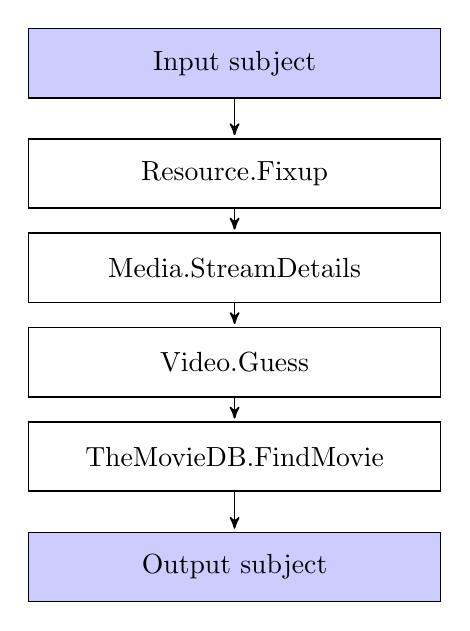
\begin{tikzpicture}[->,>=stealth',shorten >=1pt,auto,node distance=2.4cm,semithick]
		\tikzstyle{every state}=[]
		 		
		\node[subject] (InputSubject) {Input subject};
	
		\node[state] [below=0.5cm of InputSubject] (ResourceFixup) {Resource.Fixup};
		\node[state] [below=0.3cm of ResourceFixup] (MediaStreamDetails) {Media.StreamDetails};
		\node[state] [below=0.3cm of MediaStreamDetails] (VideoGuess) {Video.Guess};
		\node[state] [below=0.3cm of VideoGuess] (TheMovieDBFindMovie) {TheMovieDB.FindMovie};
		
		\node[subject] [below=0.5cm of TheMovieDBFindMovie] (OutputSubject) {Output subject};
			 		
		% paths
		\path (InputSubject) edge node {} (ResourceFixup);		
		
		\path (ResourceFixup) edge node {} (MediaStreamDetails);
		\path (MediaStreamDetails) edge node {} (VideoGuess);
		\path (VideoGuess) edge node {} (TheMovieDBFindMovie);
		
		\path (TheMovieDBFindMovie) edge node {} (OutputSubject);
	\end{tikzpicture}
	\caption{The sequential pipeline created by only giving URL}
	\label{figure:alien-linear-pipeline}
\end{figure}

\begin{figure}
	\centering
	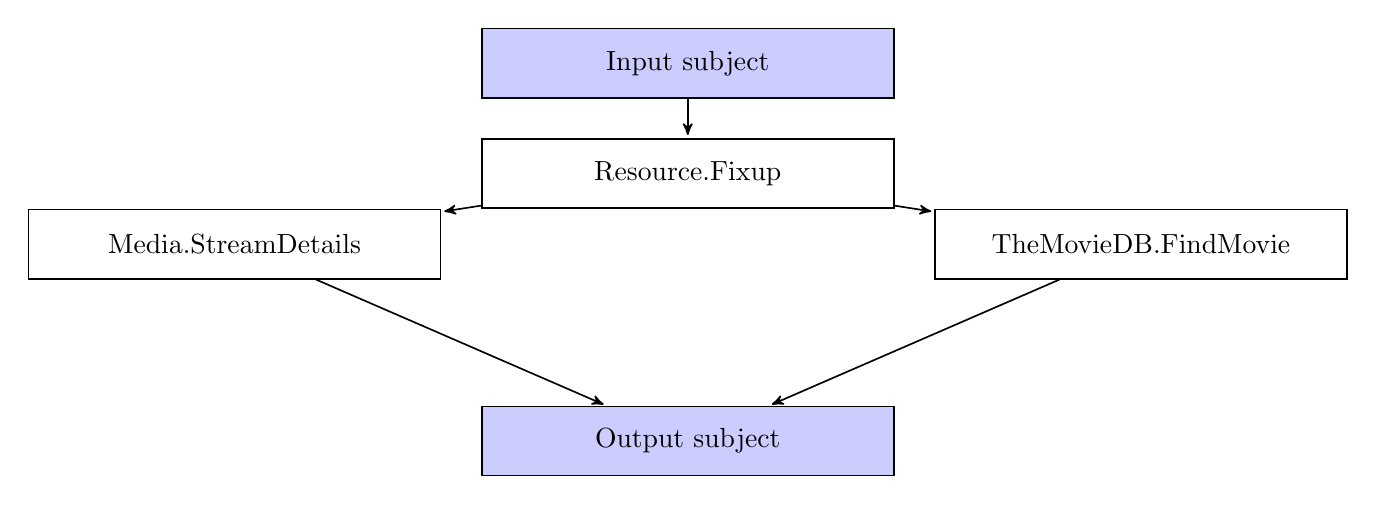
\begin{tikzpicture}[->,>=stealth',shorten >=1pt,auto,node distance=2.4cm,semithick]
		\tikzstyle{every state}=[]
		 		
		\node[subject] (InputSubject) {Input subject};
	
		\node[state] [below=0.5cm of InputSubject] (ResourceFixup) {Resource.Fixup};
		\node[state] [below left=0.0cm and 0.5cm of ResourceFixup] (MediaStreamDetails) {Media.StreamDetails};
		\node[state] [below right=0.0cm and 0.5cm of ResourceFixup] (TheMovieDBFindMovie) {TheMovieDB.FindMovie};
		
		\node[subject] [below=2.5cm of ResourceFixup] (OutputSubject) {Output subject};
			 		
		% paths
		\path (InputSubject) edge node {} (ResourceFixup);
		
		\path (ResourceFixup) edge node {} (MediaStreamDetails);
		\path (ResourceFixup) edge node {} (TheMovieDBFindMovie);
		
		\path (MediaStreamDetails) edge node {} (OutputSubject);		
		\path (TheMovieDBFindMovie) edge node {} (OutputSubject);
	\end{tikzpicture}
	\caption{The parallel pipeline created by only giving URL and content}
	\label{figure:alien-parallel-pipeline}
\end{figure}

Each of these tasks can be further split up in multiple stages, each stage can have any number of requirement task which Heimdall will fulfill before running each stage. A task is considered finished when all stages has run. A task may have a result which is piped to requiring tasks.

\section{Coding Style}
The coding style in Heimdall follows that which is set forth in PEP-8 \cite{pep-8}.
There are a few exceptions though, namely, json styled object and list indentations
are allowed. As an example:

\begin{lstlisting}[language=Python]
foobar = {
    "foo": "bar",
    "bar": "foo"
}

foobar = [
    1,
    2
]
\end{lstlisting}

\bibliography{heimdall}

\end{document}
